%!TEX root = uw-ethesis.tex
% chktex-file 46 (ignore warnings about $...$)
% chktex-file 24 (ignore \label warning)

\chapter{\texorpdfstring{Sampling-Based Motion Planning with $\mu$-Calculus Specifications without Steering}{Sampling-Based Motion Planning with mu-Calculus Specifications without Steering}}
\label{chap:sstpaper}

This chapter presents the work published by the author of this thesis in~\cite{Larocque2018}.

%%%%%%%%%%%%%%%%%%%%%%%%%%%%%%%%%%%%%%%%%%%%%%%%%%%%%%%%%%%%%%%%%%%%%%%%%%%%%%%%
%%%%%%%%%%%%%%%%%%%%%%%%%%%%%%%%%%%%%%%%%%%%%%%%%%%%%%%%%%%%%%%%%%%%%%%%%%%%%%%%
\section{Introduction}
%%%%%%%%%%%%%%%%%%%%%%%%%%%%%%%%%%%%%%%%%%%%%%%%%%%%%%%%%%%%%%%%%%%%%%%%%%%%%%%%
%%%%%%%%%%%%%%%%%%%%%%%%%%%%%%%%%%%%%%%%%%%%%%%%%%%%%%%%%%%%%%%%%%%%%%%%%%%%%%%%

Motion planning in complex environments has seen a shift towards using sampling-based planning algorithms. By using a predetermined sampling scheme, a random snapshot of the workspace can be taken and incrementally improved upon without any prior knowledge of the environment. Furthermore, combining sampling-based motion planning with temporal logic specifications grants users a much more sophisticated toolbox of high-level behaviors that can be specified. 

Temporal logics present a means of formally expressing high-level specifications for use in various problems in mathematics, robotics, and computer science. In particular, temporal logic specifications are well-suited for motion planning problems, allowing a user-defined specification to describe the desired behavior of an autonomous vehicle or robot(e.g., ~\cite{Lin2014, Wolff2014,Doherty2013}). The modal \mucalc{} is a highly expressive temporal logic which permits more diverse and complex specifications than the most widely used temporal logics, including \gls{ltl}, \gls{ctl}, and extensions thereof. On the other hand, it is typically much easier to understand \gls{ltl} specifications at a glance, whereas \mucalc{} formulas can be much more difficult to intuit. For example, the \gls{ltl} formula for reachability is $\Diamond p$, which is equivalent to the more complicated \mucalc{} expression $\mu X.(p \lor \Diamond X)$. The added complexity of \mucalc{} formulas is not without benefit, however, as a major advantage lies in its predisposition for simple model checking. While \gls{ltl} specifications are a useful tool for high-level planning, they must usually be translated into automata for the purposes of model checking. The equivalent \mucalc{} specification, however, can be checked directly without any intermediate steps via the Tarski-Knaster fixed point theorem~\cite{Emerson1999, Tarski1955}.

In this work, a fragment of the full \mucalc{} called deterministic \mucalc{}~\cite{Karaman2009} is used, allowing for efficient model checking while maintaining the ability to specify complex tasks. Some such specifications include reaching a goal while avoiding obstacles, and a property known as liveness, which involves satisfying one or many propositions infinitely often. Furthermore, using the model checking algorithm discussed in \autoref{chap:sstpaper:main}, it is possible to formally synthesize a control policy that provably satisfies a given deterministic \mucalc{} specification.


%%%%%%%%%%%%%%%%%%%%%%%%%%%%%%%%%%%%%%%%%%%%%%%%%%%%%%%%%%%%%%%%%%%%%%%%%%%%%%%%
%%%%%%%%%%%%%%%%%%%%%%%%%%%%%%%%%%%%%%%%%%%%%%%%%%%%%%%%%%%%%%%%%%%%%%%%%%%%%%%%
\section{Problem Formulation}
%%%%%%%%%%%%%%%%%%%%%%%%%%%%%%%%%%%%%%%%%%%%%%%%%%%%%%%%%%%%%%%%%%%%%%%%%%%%%%%%
%%%%%%%%%%%%%%%%%%%%%%%%%%%%%%%%%%%%%%%%%%%%%%%%%%%%%%%%%%%%%%%%%%%%%%%%%%%%%%%%

Consider a time-invariant continuous dynamical control system given by the differential equation
\begin{align}\label{dynsys}
    \dot x(t) = f(x(t),u(t)), \hspace{4mm} x(0) = x_0
\end{align}
where $x \in \R^n$ is the state, $u \in \R^m$ is the control input, and 
$f: \R^n \times \R^m \to \R^n$ is a locally Lipschitz function. Let $\Pi$ be a set of {\em atomic propositions}, which are the simplest form of declarative statements that are either true or false. Lastly, let $L: \R^n \to 2^\Pi$ be a labeling function which assigns to a state all of the atomic propositions that it satisfies.

The goal is to design a controller such that the possibly infinite state trajectory $x(t)$ satisfies a given temporal logic specification, $\Phi$. We choose to work with deterministic \mucalc{} for reasons discussed in \autoref{prelims:deterministic_mucalc}. It is important to note that model checking of the temporal logic specification must be performed on a finite model of the dynamical system. To this end, a sampling-based motion planner is used to generate a discretization of the set of possible trajectories from the initial condition in the form of a Kripke structure.

\begin{defn}
    A Kripke structure $K = (S, \{s_0\}, R, \L)$ \emph{models} the dynamical control system (\ref{dynsys}) with initial state $x(0)$ if (i) $S \subseteq \R^n$; (ii) $s_0 = x(0) \in S$; (iii) $(s,s') \in R$ only if there exist $t_0, t_1 \in \R$, $t_1 > t_0$, and a control signal $u: [t_0, t_1] \to \R^m$ such that $s = x(t_0) \in \R^n$ and $s' = x(t_1) = x(t_0) + \int_{t_0}^{t_1} f(x(t), u(t)) dt$; (iv) $\L(s) = L(s)$ for all $s \in S$.
\end{defn}

This definition provides a concrete way of evaluating whether or not a Kripke structure sufficiently models any given dynamical system. We use this definition in the problem statement that follows.


\subsection{Problem Statement}

A precise formulation of the problem to be solved can now be made. We seek to use a dynamical control system together with the notions of Kripke structures and deterministic \mucalc{} specifications, the aim being to determine whether a given specification is satisfied by a Kripke structure that models the dynamical control system.

\begin{defn}
    A continuous-time dynamical control system of the form (\ref{dynsys}) is said to satisfy a deterministic \mucalc{} specification $\Phi$ at some initial state $x_0$ if and only if there exists a Kripke structure 
    $K^* = (S^*,\{x_0\},R^*,\mathcal{L}^*)$ modeling the system, and such that $x_0 \in \brackets{\Phi}_{K^*}$.
\end{defn}

In contrast to~\cite{Karaman2009}, we allow the dynamical control system to be continuous in time. The problem statement is as follows:

\begin{problem}
    Given a continuous-time dynamical control system (\ref{dynsys}) with initial state $x_0$ and a deterministic \mucalc{} formula $\Phi$, return a control policy $u$ which gives rise to a trajectory satisfying $\Phi$ obtained from a Kripke structure that models the system, or return failure if such a trajectory is not found.
\end{problem}

%%%%%%%%%%%%%%%%%%%%%%%%%%%%%%%%%%%%%%%%%%%%%%%%%%%%%%%%%%%%%%%%%%%%%%%%%%%%%%%%
%%%%%%%%%%%%%%%%%%%%%%%%%%%%%%%%%%%%%%%%%%%%%%%%%%%%%%%%%%%%%%%%%%%%%%%%%%%%%%%%
\section{Kripke Structures and Model Checking}\label{chap:sstpaper:main}
%%%%%%%%%%%%%%%%%%%%%%%%%%%%%%%%%%%%%%%%%%%%%%%%%%%%%%%%%%%%%%%%%%%%%%%%%%%%%%%%
%%%%%%%%%%%%%%%%%%%%%%%%%%%%%%%%%%%%%%%%%%%%%%%%%%%%%%%%%%%%%%%%%%%%%%%%%%%%%%%%

The main goal of this work is to design an algorithm that finds near-optimal trajectories satisfying a given temporal logic specification without relying on an \gls{obvp} (steering function). The motivation for such an algorithm is that in a differentially constrained system, finding an optimal trajectory between two states is difficult in general. Some research has been done to first linearize system dynamics to find a solution to the BVP~\cite{Webb2013}, while others have found some success in numerical solutions to BVPs with nonlinear dynamics using sequential quadratic programming~\cite{Xie2015}. However, neither approach fully addresses the crux of the problem: some planning problems, such as systems simulated on a physics engine, allow only forward propagation. We opt to use the asymptotically optimal variant of \gls{sst} called \gls{sst}* by Li et al.~\cite{Li2016} which does not require a steering function to plan high-quality trajectories.


\subsection{\texorpdfstring{Model Checking with \muCalc{} Specifications}
                           {Model Checking with mu-Calculus Specifications}}

%Talk about running SST*
It is necessary to determine whether or not the \mucalc{} specification $\Phi$ is satisfied during the incremental tree expansion (refining the discretized state space) with \gls{sst}*. To perform such a verification, we will use a local model checking algorithm tailored specifically to run efficiently for deterministic \mucalc{}. The procedure requires as input a Kripke structure, $K$, the \mucalc{} specification, $\Phi$, an initial state, $s$, and the subformula to be checked in the current execution, $\phi$. We further require a function $\texttt{succ}(s)$, which returns all states in $K$ which may be reached from $s$ via one relation (edge of the tree), and $\texttt{BoundFormula}(X)$, which maps the input variable $X$ to the subformula of $\Phi$ of the form $\sigma X.\psi$, that is, the smallest subformula that binds the variable $X$ to a least or greatest fixed-point operator. Note that the first two arguments of \texttt{ModelCheck} are omitted in recursive calls for brevity as they remain unchanged. The local model checking algorithm presented here is based on Algorithm 3 presented in~\cite{Karaman2009}.

\begin{algorithm}
\caption{\texttt{ModelCheck}$(K, \Phi, s, \phi)$}
\label{alg:modelchecking}
\begin{algorithmic}[1]
    \Switch{$\phi$}
        \Case{$p$ where $p \in \Pi$}
            \Return{$p \in \L(s)$}
        \EndCase{}
        \Case{$\lnot p$ where $p \in \Pi$}
            \Return{$p \notin \L(s)$}
        \EndCase{}
        \Case{$p \land \varphi$}
            \Return{$p \land \texttt{ModelCheck}(s, \varphi)$}
        \EndCase{}
        \Case{$\lnot p \land \varphi$}
            \Return{$\lnot p \land \texttt{ModelCheck}(s, \varphi)$}
        \EndCase{}
        \Case{$\psi \lor \varphi$}
            \Return{$\texttt{ModelCheck}(s, \psi) \lor \texttt{ModelCheck}(s, \varphi)$}
        \EndCase{}
        \Case{$\Diamond \varphi$}
            \For{$s' \in \texttt{succ}(s)$}
                \If{$\texttt{ModelCheck}(s', \varphi)$}
                    \Return{\texttt{True}}
                \EndIf{}
            \EndFor{}
            \Return{\texttt{False}}
        \EndCase{}
        \Case{$\sigma X.\varphi$ where $\sigma \in \{ \mu, \nu \}$}
            \State{$\texttt{set} \gets \texttt{set} \cup \{ (s,\varphi) \}$}
            \State{$\texttt{value} \gets \texttt{ModelCheck}(s, \varphi)$}
            \State{$\texttt{set} \gets \texttt{set} \setminus \{ (s,\varphi) \}$}
            \Return{\texttt{value}}
        \EndCase{}
        \Case{$X$ where $X \in \Var$}
            \If{$(s, \text{\texttt{BoundFormula$(X)$}}) \in \texttt{set}$}
                \Switch{\texttt{BoundFormula$(X)$}}
                    \Case{$\mu X.\varphi$}
                        \Return{\texttt{False}}
                    \EndCase{}
                    \Case{$\nu X.\varphi$}
                        \Return{\texttt{True}}
                    \EndCase{}
                \EndSwitch{}
            \Else{}
                \Return{\texttt{ModelCheck$(s, \text{\texttt{BoundFormula$(X)$}})$}}
            \EndIf{}
        \EndCase{}
    \EndSwitch{}
\end{algorithmic}{}
\end{algorithm}

\autoref{alg:modelchecking} is a recursive function which returns a boolean value without having to create any intermediary graphs unlike the proposed {\em incremental\/} model checking algorithms from~\cite{Emerson1999} and~\cite{Karaman2009}, and also without the need for generating an automaton on which to perform model checking, unlike when using \gls{ltl}, for example. Since model checking will be performed on a very small abstracted Kripke structure, using the local, non-incremental model checking algorithm is sufficient. The algorithm presented here is based on a similar algorithm from~\cite{Schneider2004}, wherein correctness is proved.

\subsection{Abstracted Kripke Structure and Planning}

The primary contribution we make is to simplify model checking over several data structures by creating an abstracted Kripke structure. We generate this new abstracted structure ${\tilde{K}_{\Pi^+(\Phi)} = (\tilde{S}, \{ \tilde{s_0} \}, \tilde{R}, \L)}$ from $p = \lvert {\Pi^+(\Phi)} \rvert$ Kripke structures of the form ${K_i = (S_i, \{ {s_i}_0 \}, R_i, \L)}, i = \{1, \mathellipsis, p \}$, generated via \gls{sst}*, where $\Pi^+(\Phi) \subseteq \Pi$ is the set of atomic propositions which appear positively in specification $\Phi$. The reason for restricting the abstracted Kripke structure to use only the positively-appearing atomic propositions is that these are the specifications we explicitly want to fulfill (e.g., reach a certain goal), as opposed to something we do not want our system to do (e.g., run into obstacles). In this way, a directed edge is added to the abstracted Kripke structure only if a trajectory in one of the $K_i$ is found to initially satisfy one atomic proposition, and reaches a state satisfying another atomic proposition, all the while ensuring any negatively-appearing atomic propositions are respected so that the associated regions of state space are avoided. If any of these conditions does not hold, the edge is not added to the graph. The planning procedure, including the generation of the abstracted Kripke structure and the model checking to be performed on this structure, is as follows.

\begin{algorithm}
\caption{\texttt{KinoSpecPlan}$(f, x_0, \Phi, \texttt{regions}, \L)$}
\label{alg:kinospecplan}
\begin{algorithmic}[1]
    \State{$\tilde{K} \gets (\{x_0\}, \{x_0\}, \emptyset, \L)$}\label{alg:kinoplan:start}
    \State{$K \gets \emptyset$}
    \State{$p \gets \texttt{length}(\texttt{regions})$}\label{alg:kinoplan:start2}
    \For{$i \in \{ 1, \ldots, p \}$}\label{alg:kinoplan:initK}
        \State{${s_i}_0 \gets \texttt{ChooseInit} (\texttt{regions}[i], x_0)$}
        \State{$K_i \gets (\{ {s_i}_0 \}, \{ {s_i}_0 \}, \emptyset, \L)$}
        \State{$K \gets K \cup \{ K_i \}$}\label{alg:kinoplan:initK2}
    \EndFor{}
    \While{$\lnot \texttt{ModelCheck}(\tilde{K}, \Phi, x_0, \Phi)$}\label{alg:kinoplan:sst}
        \For{$i \in \{1, \ldots, p\}$}
            \State{$K_i \gets$ SST*$(K_i)$}\label{alg:kinoplan:sst2}
        \EndFor{}
        \State{$\tilde{K} \gets$ \texttt{AbstractUpdate}$(\tilde{K}, K)$}\label{alg:kinoplan:abstract}
    \EndWhile{}
    \Return{\texttt{ConstructPath}$(\tilde{K}, K)$}\label{alg:kinoplan:end}
    % \State $x \gets x_0$
    % \While{\texttt{True}}
    %     \State $A, B \gets \texttt{Linearize}(f, t, path)$
    %     \State $K_{LQR} \gets$ LQR$(A,B,Q,R)$
    %     \State $\texttt{e} \gets x-$
\end{algorithmic}{}
\end{algorithm}

The $\texttt{KinoSpecPlan}$ algorithm takes as input the dynamics $f$ from (\ref{dynsys}), the initial condition $x_0$, the deterministic \mucalc{} specification $\Phi$, an array called \texttt{regions} containing $p$ subsets of the state space (one for each positively-appearing atomic proposition in $\Phi$), and the labeling function $\L$. The function \texttt{ChooseInit} samples a state from the input region to use as the initial state for Kripke structure $K_i$, or $x_0$ if it exists in the given region. \gls{sst}* takes a Kripke structure and incrementally grows the structure using forward propagation, thereby updating its set of states and relations. \texttt{AbstractUpdate} verifies the existence of any paths spanning from one region to another in the list $K$ of all Kripke structures. If so, the corresponding relation is added to the list of relations maintained in the abstracted Kripke structure $\tilde{K}$. Furthermore, the first time it is run, \texttt{AbstractUpdate} adds the necessary states from the initial states of each of the $K_i$ to its own set of states. Using the abstracted Kripke structure and the list of all Kripke structures, \texttt{ConstructPath} creates a single time-parameterized state trajectory along the least-cost path satisfying $\Phi$, where each individual candidate path from the Kripke structures is combined head-to-tail as necessary. 
% Finally, \texttt{Linearize} takes in the function for the dynamics of the system, $f$, a time $t$, and \texttt{path}, and returns the matrices $A$ and $B$ of the linearization $\dot x \approx Ax + Bu$ centered at \texttt{path}(t). 

In essence, the algorithm works as follows. First, the abstracted Kripke structure $\tilde{K}$ is initialized with only the initial condition and an empty set of relations, and $K$, the list of Kripke structures, is initialized to be empty (lines~\ref{alg:kinoplan:start}--\ref{alg:kinoplan:start2}). In lines~\ref{alg:kinoplan:initK}--\ref{alg:kinoplan:initK2}, the for-loop initializes each Kripke structure $K_i$, $i \in \{ 1,\ldots,p \}$, to be the trivial graph consisting only of the initial condition ${s_i}_0$, which is chosen from among any of the states in the proposition region $\brackets{\pi_i}$ associated with atomic proposition $\pi_i \in \Pi^+$; that is, the initial node ${s_i}_0$ of $K_i$ satisfies $\pi_i \in \L({s_i}_0)$.

Next, each Kripke structure is expanded in parallel using the \gls{sst}* motion planning algorithm (lines~\ref{alg:kinoplan:sst}--\ref{alg:kinoplan:sst2}).
The abstracted Kripke structure $\tilde{K}_{\Pi^+}$ is then updated in line~\ref{alg:kinoplan:abstract} so that each of its $p$ nodes $\tilde{s_i} \in \tilde{S}$ corresponds to a positively-appearing atomic proposition, so $\pi_i \in \L(\tilde{s_i})$, $i \in \{ 1, \ldots, p \}$ (this particular procedure only occurs the first time \texttt{AbstractUpdate} is executed). 
The crucial aspect of this step is that the relations in $\tilde{R}$ are also updated, and relation $(\tilde{s_a}, \tilde{s_b})$ is added if and only if there exists a path in the Kripke structure $K_a$ from ${s_a}_0 \in S_a$ to a node ${s_b} \in S_a$ satisfying $\pi_b \in \L(s_b)$.

The deterministic \mucalc{} model checking algorithm \texttt{ModelCheck} verifies whether the abstracted Kripke structure $\tilde{K}$ satisfies the given specification, $\Phi$. If the specification is not satisfied, the while-loop repeats lines~\ref{alg:kinoplan:sst}--\ref{alg:kinoplan:abstract}. Once the specification is found to be satisfied by the abstracted Kripke structure $\tilde{K}$, a time-parameterized trajectory is created from the combination of the best paths found among the relevant Kripke structures $K_i$ (line~\ref{alg:kinoplan:end}).

Note that in order to use the path returned by \autoref{alg:kinospecplan}, we track it using an LQR controller obtained by linearizing the dynamical system~(\ref{dynsys}) at the current state. The state error can then be obtained and the appropriate feedback control can be applied until the next time step, at which point the LQR algorithm must be run again. 

\subsection{LQR Tracking}\label{section:lqr}

Once the abstracted Kripke structure $\tilde{K}_{\Pi^+(\Phi)}$ is generated and the model checking algorithm confirms the satisfaction of the \mucalc{} specification $\Phi$, it is necessary to connect the candidate trajectories from the various $K_i$ structures. Accordingly, for all paths in $\tilde{K}_{\Pi^+(\Phi)}$ satisfying $\Phi$, the corresponding candidate trajectories in the $K_i$ structures are bridged together within the appropriate proposition region, i.e., the region in state space where every state $x$ satisfies a particular proposition $p \in \Pi^+(\Phi)$. To do so, we apply an LQR controller as in~\cite{Tedrake2009}.

First, the dynamical system is linearized to be of the form $\dot x = Ax + Bu$. We then define the quadratic cost function over the time interval $[ t_0, t_1 ]$ to be
\begin{equation}
    J = \int_{t_0}^{t_1} \left( {\bar x}^\top Q {\bar x} + {\bar u}^\top R {\bar u} \right)dt
\end{equation}
where $Q$ is a symmetric positive semi-definite state cost matrix, $R$ is a symmetric positive definite control cost matrix, the tracking error is $\bar x = x - x_c$ where $x_c$ is the time-parameterized total candidate trajectory found by patching together the individual candidate trajectories in sequence, and $\bar u = u - u_c$ where $u_c$ is the corresponding control signal for $x_c$. To proceed, the steady-state solution $P$ to the continuous algebraic Ricatti equation (CARE)
\begin{equation}
    A^\top P + PA - PBR^{-1}B^\top P + Q = 0 
\end{equation}
must be found. The feedback control is then given by $u = u_c - K{\bar x}$, where $K = R^{-1}B^\top P$.

% In order to join the various trajectories which together satisfy the given \mucalc{} proposition $\Phi$, the LQR controller is applied to track each trajectory sequentially. Given the exact time and location of states along a time-parameterized path $\gamma_1$ from Kripke structure $K_{\gamma_1}$, the LQR controller uses the error between the expected next state (from the tracked trajectory), $s_\gamma$, and the actual current state, $s_{cur}$. When the end of the path $\gamma_1$ is reached, the next path $\gamma_2$ from Kripke structure $K_{\gamma_2}$ is followed, and so on until a path is formed satisfying specification $\Phi$. The error along each path $\gamma_i$ is then given by $e_i(t) = s_{\gamma_i}(t) - s_{cur}(t)$, and tracking is accomplished by applying control $u_i = -Ke_i(t)$ along the trajectory.


%%%%%%%%%%%%%%%%%%%%%%%%%%%%%%%%%%%%%%%%%%%%%%%%%%%%%%%%%%%%%%%%%%%%%%%%%%%%%%%%
%%%%%%%%%%%%%%%%%%%%%%%%%%%%%%%%%%%%%%%%%%%%%%%%%%%%%%%%%%%%%%%%%%%%%%%%%%%%%%%%
\section{Example}
%%%%%%%%%%%%%%%%%%%%%%%%%%%%%%%%%%%%%%%%%%%%%%%%%%%%%%%%%%%%%%%%%%%%%%%%%%%%%%%%
%%%%%%%%%%%%%%%%%%%%%%%%%%%%%%%%%%%%%%%%%%%%%%%%%%%%%%%%%%%%%%%%%%%%%%%%%%%%%%%%

\begin{figure}
    \centering
    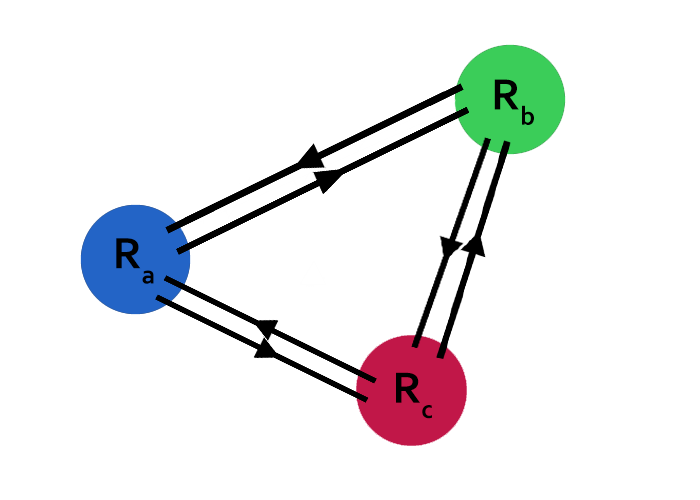
\includegraphics{./figures/abstract_kripke.png}
    \caption[Abstracted Kripke Structure]{Representation of the abstracted Kripke structure of the provided example. This structure is verified with the local model checking algorithm (\autoref{alg:modelchecking}) to ensure satisfaction of the deterministic \mucalc{} specification.} 
\label{fig:abs_kripke}
\end{figure}

To demonstrate the effectiveness of our method, we provide the following pertinent example. We use continuous double integrator dynamics on two spatial dimensions, resulting in a 4D state space. State and control vectors take the form
\begin{equation}
    \vec{x} =  \begin{bmatrix}
                    x \\
                    y \\
                    \dot x \\
                    \dot y
                \end{bmatrix},
    \ \vec{u} =  \begin{bmatrix}
                    u_x \\
                    u_y
                \end{bmatrix}
\end{equation}
and the dynamical system is given by
\begin{equation}
    \dot{\vec{x}} = %\begin{pmatrix}
                        \begin{bmatrix}
                            0 & 0 & 1 & 0 \\
                            0 & 0 & 0 & 1 \\
                            0 & 0 & 0 & 0 \\
                            0 & 0 & 0 & 0 \\
                        \end{bmatrix} \vec{x} +
                        \begin{bmatrix}
                            0 & 0 \\
                            0 & 0 \\
                            1 & 0 \\
                            0 & 1  
                        \end{bmatrix} \vec{u},
                    %\end{pmatrix}
\end{equation}
with initial condition $\vec{x}_0 = [100, 400, 0, 0]$.
We choose the cost function for \gls{sst}* to be the duration of the trajectory, T, along with a control cost term, with cost matrix $R_{sst}$:
\begin{equation}
    J_{SST} = \int_0^\top \left( 1 + u^\top R_{sst} u \right ) dt.
\end{equation}
% Define atomic propositions $a,b,$ and $c$ to be true for state $s$ if and only if $s \in R_a$, or $s \in R_b$, or $s \in R_c$, respectively,
The specification we wish to satisfy is to visit three distinct regions of the state space,
$R_a, R_b$, and $R_c$ infinitely often while avoiding the obstacle regions collectively called $R_o$. Define atomic propositions $p_i$, $i \in \{a, b, c, o\}$, such that ${p_i} \in \mathcal{L}(s)$ if and only if $s \in R_i$. We write the deterministic \mucalc{} formula $\Phi$ as follows
\begin{align*}
    \mu M.[  (\lnot o \land \Diamond M) \lor \\
        \nu W.\{
            ( a &\land \mu X.[\lnot o \land ( ((b \lor c) \land W) \lor \Diamond X)] ) \lor \\
            ( b &\land \mu Y.[\lnot o \land ( ((a \lor c) \land W) \lor \Diamond Y)] ) \lor \\
            ( c &\land \mu Z.[\lnot o \land ( ((a \lor b) \land W) \lor \Diamond Z)] ) \} ].
\end{align*}

Upon running \gls{sst}* in three parallel instances starting in the center of each proposition's associated region in state space, we obtained \autoref{fig:all_trees}. Note that there are six candidate trajectories, each representing the best path from one region to another in terms of the cost, $J_{SST}$. In general, for $p$ positively-appearing atomic propositions in the {\mucalc{}} specification, $p$ trees are incrementally updated in parallel, and we search for ${p-1}$ candidate trajectories for each tree.

The model checking algorithm ensures that at least one cycle of length three may be formed in the abstracted Kripke structure, which itself is constructed with three nodes (one for each proposition region), and whose directed edges represent the candidate trajectories that begin in one proposition region and end in another one. The procedure was run until all six candidate trajectories successfully reached their appropriate goal regions, allowing for the abstracted Kripke structure to be fully connected\footnote{This was done in order to compare the cost associated with each direction of the possible 3-cycle, although \autoref{alg:kinospecplan} as it is written would return as soon as any satisfactory path is found.}. The resulting structure contains two infinite paths satisfying proposition $\Phi$ above, noting that the initial condition is situated in the blue region: (i)\ head to the green region first, then the burgundy region, and returning to the blue region to repeat, or (ii)\ head to the burgundy region first, then the green region, and repeating upon returning to the blue region.

In order to determine which of the cycles to take, a simulation is run using the LQR controller discussed in \autoref{section:lqr}, tracking each of the proposed paths and bridging the gap between the end of one trajectory and the beginning of another. The state-cost matrix $Q$ was set to $\texttt{diag}(25, 25, 25, 25)$ and the control-cost matrix $U$ was chosen to be $\texttt{diag}(1, 1)$. Using total cost to determine the better of the two proposed solutions, it is found that option (i)\ results in a faster circuit between the three regions. See \autoref{fig:sol}.


\begin{figure}
    \centering
    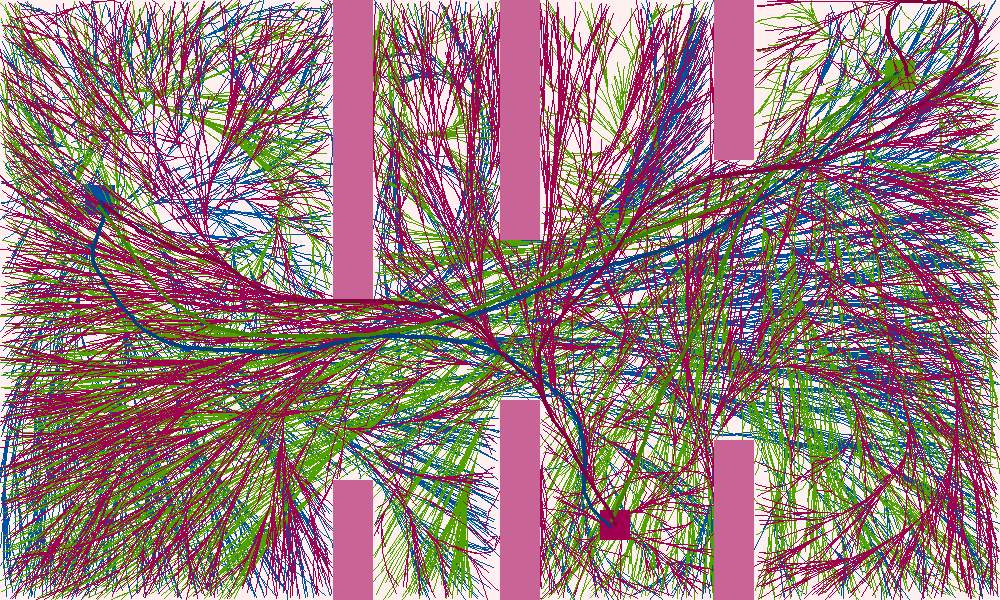
\includegraphics[scale=0.61]{./figures/doubleint2.png}
    \caption[Double Integrator Example --- Three Trees using SST*]{\gls{sst}* is performed three times, producing a Kripke structure for each of the regions shown here in blue (left), burgundy (bottom center), and green (top right). Obstacles are represented as pink rectangles. The color of each line matches the color of the region of the Kripke structure to which it belongs, and the bolded curves are the lowest-cost trajectories that reach another region.} 
    \label{fig:all_trees}
\end{figure}

\begin{figure}
    \centering
    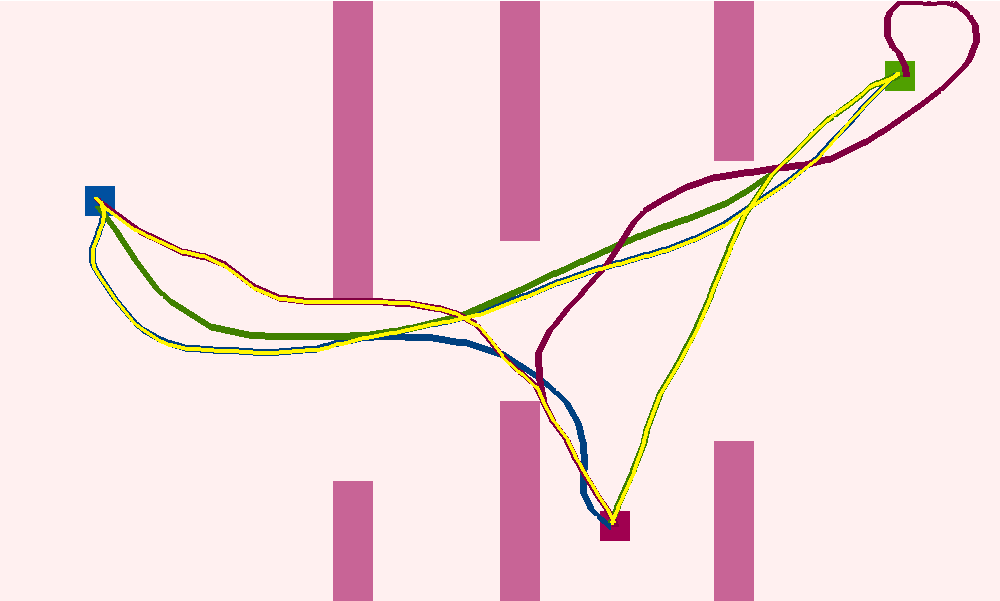
\includegraphics[scale=0.61]{./figures/doubleint2-good-lqr.png}
    \caption[Double Integrator Example --- Simulation Results]{The six candidate trajectories are shown, where curves of the same color are selected from the same Kripke structure. The solution trajectory is shown in yellow, starting in the center of the blue region and tracking the infinite path with least cost that satisfies specification $\Phi$.} 
\label{fig:sol}
\end{figure}


%    \begin{figure}[thpb]
%       \centering
%       \framebox{\parbox{3in}{We suggest that you use a text box to insert a graphic (which is ideally a 300 dpi TIFF or EPS file, with all fonts embedded) because, in an document, this method is somewhat more stable than directly inserting a picture.
% }}
%       %\includegraphics[scale=1.0]{figurefile}
%       \caption{Inductance of oscillation winding on amorphous
%        magnetic core versus DC bias magnetic field}
%       \label{figurelabel}
%    \end{figure}
   
